A camera was needed for the UAV to visually identify the fiducial marker. The gimbal we used was designed for a GoPro Hero 3, but the latency of GoPro video streams meant that a GoPro would be unusable. Therefore, alternative cameras modules were used - namely, the IMX219-160 wide-angle camera and the Google Coral camera module. These allow for near realtime video streaming and analysis with the given companion boards. Kjartan and Joshua iteratively designed and tested multiple camera cases (shown in Figure \ref{fig:camera_case_iterations}) to properly mount the camera modules in the gimbal's GoPro holder. We then 3D printed them and installed them on the drones. According to the gimbal's design, the lens of the GoPro is supposed to be slightly off-center in both the horizontal and vertical directions. In early versions of the camera cases, the camera modules were positioned in the same place. This meant that the modules would have to be rotated 90 degrees in order to allow their data cables to extend out of a small slit the case without obstruction. The video feed was then rotated back before video analysis. However, in later revisions of the camera cases, we have positioned the lenses closer to the center of rotation in the pan and tilt axes. This allows room for the camera's ribbon cable to extend out of the bottom of the camera case without obstruction, creates a neater and more reliable system, and eliminates the need for rotating the video feed in software. The final camera modules are shown in Figures \ref{fig:nano_case} and \ref{fig:coral_case}. They were designed in OpenSCAD and all .stl and .scad files are available freely on Thingiverse \cite{camera_thingiverse}.

\begin{figure}
    \centering
    \includegraphics[width=0.7\textwidth, angle=180]{images/camera_module_iterations.JPG}
    \caption{Iterations of the camera case design The camera module was gradually moved to the side and oriented upwards in order to allow the best fit in the gimbal.}
    \label{fig:camera_case_iterations}
\end{figure}

\begin{figure}
    \begin{subfigure}[b]{0.48\textwidth}
        \centering
        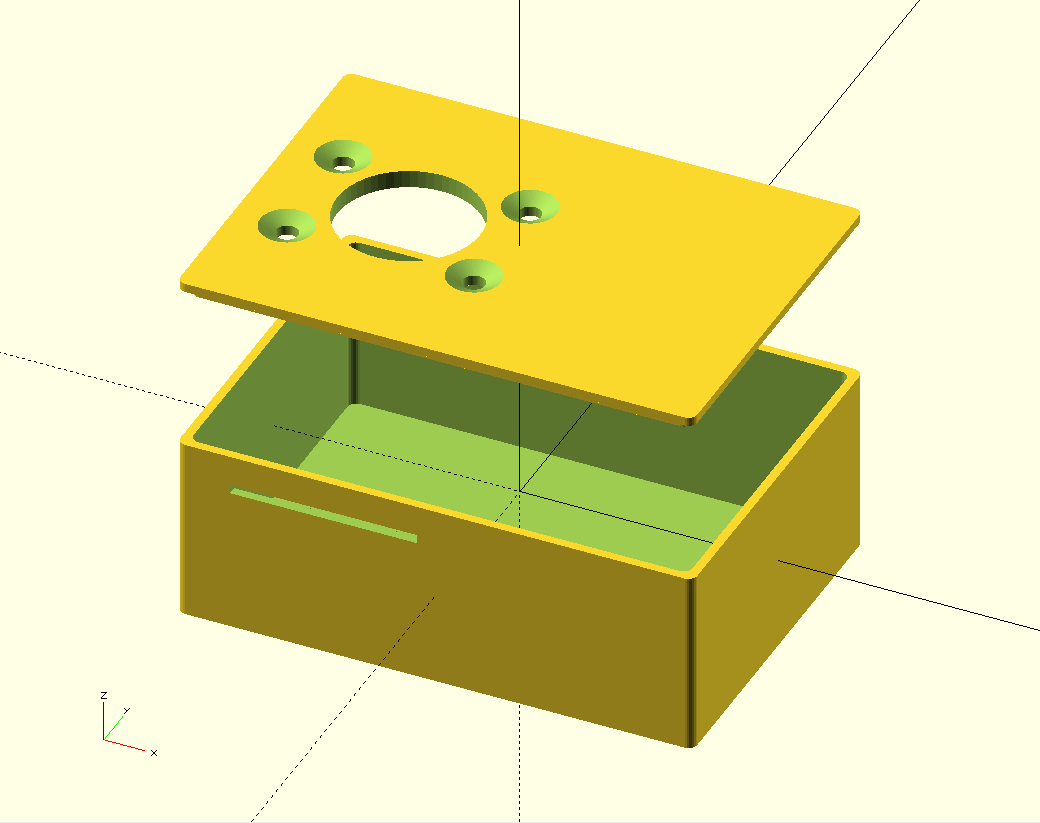
\includegraphics[width=\textwidth]{images/nano_case.png}
        \caption{The case for the IMX219-160 camera module.}
        \label{fig:nano_case}
    \end{subfigure}
    \begin{subfigure}[b]{0.48\textwidth}
        \centering
        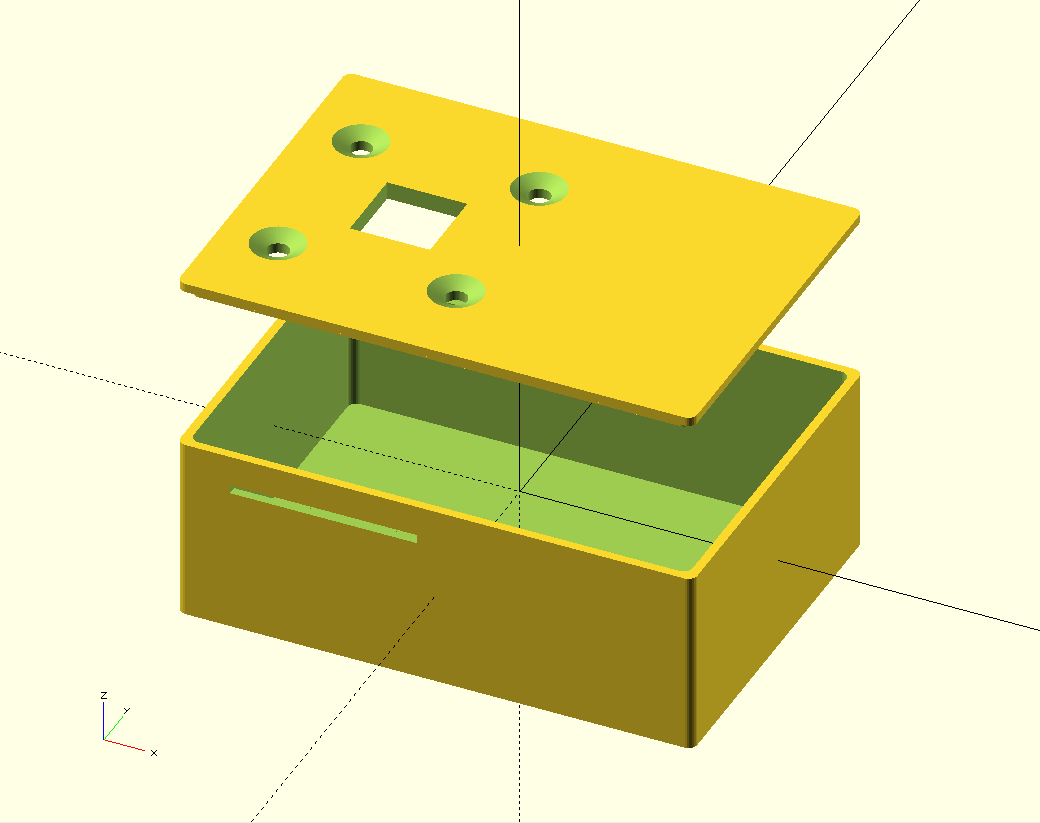
\includegraphics[width=\textwidth]{images/coral_case.png}
        \caption{The case for the Google Coral camera module.}
        \label{fig:coral_case}
    \end{subfigure}
    \caption{Cases to allow the alternative camera modules to fit into the gimbal's GoPro mount. The camera modules mount to the front with screws, and the front simply presses into the back. A slit allows the camera's ribbon cable to exit the bottom of the case.}
\end{figure}



% In order to use the module, we designed an empty camera case based on the dimensions of the Hero 3 and put the module inside the case. Four screw holes were added to the top cover of the case for the module to be screwed into, and a hole in the middle of the screw holes for the lens to go through. Enclosures were added to the case to snap the top cover and the case together. A component of the gimbal that would fasten a GoPro Hero 3 to the gimbal was removed so we could use our case instead, and because the component would be in the way of the camera's vision. We used Fusion 360 to design the case, and used Ultimaker Cura to slice the model for 3D printing. After we had 3D printed the case and tested the camera, we came to the conclusion that a much wider lens would be more optimal. We designed a new top cover but did not redesign the rest of the case since the only thing we were changing was a new camera module. 